% !TeX root = document.tex
\subsection{Базові алгоритми масштабування зображень}
Для повноцінної та об'єктивної оцінки ефективності розробленого алгоритму необхідно мати класичні методи для порівняння, тому розглянемо існуючі рішення для задачі масштабування зображень:

\begin{enumerate}
\item{Метод найближчого сусіда}
\begin{itemize}
	\item Нові значення пікселів отримуються шляхом вибору значення одного з чотирьох найближчих пікселів (з точки зору евклідової відстані).
	\item Пікселі дублюються (при збільшенні масштабу) або видаляються (при зменшенні масштабу).
	\item \underline{Нові значення} не вводяться в зображення.
	\item \underline{Відсутність інтерполяції} означає, що краї залишаються різкими.
\end{itemize}

\begin{figure}[h!]
	\centering
	% Заміни nearest.png на реальну назву твого файлу
	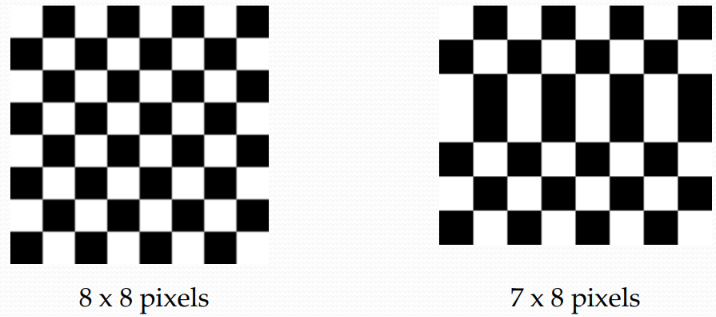
\includegraphics[width=0.6\textwidth]{figures/nearest}
\end{figure}

\newpage
\item{Білінійна інтерполяція}
\begin{itemize}
	\item До уваги беруться чотири пікселі околу.
	\item Нове значення пікселя обчислюється за допомогою лінійної комбінації навколишніх пікселів.
	\item Чим ближче знаходиться піксель в околі, тим більший вплив він має на результуюче значення.
	\item \underline{Нові значення} вводяться в зображення.
	\item \underline{Краї пом'якшуються} через лінійну інтерполяцію.
\end{itemize}

\begin{figure}[h!]
	\centering
	% Заміни bilinear.png на реальну назву твого файлу
	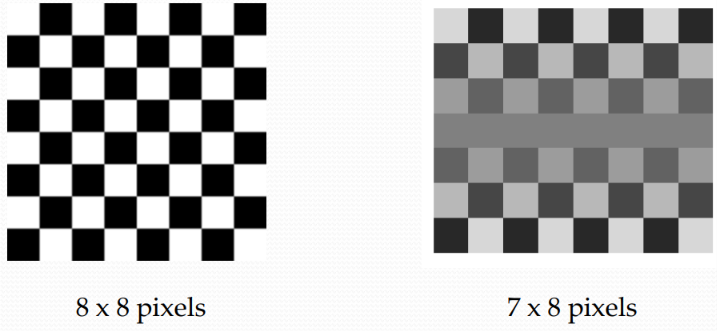
\includegraphics[width=0.6\textwidth]{figures/bilinear}
\end{figure}

\item{Бікубічна інтерполяція}
\begin{itemize}
	\item До уваги беруться шістнадцять пікселів околу.
	\item Нове значення пікселя обчислюється за допомогою кубічної функції навколишніх пікселів:
	\begin{equation*}
		f(x) = a \cdot x^3 + b \cdot x^2 + c \cdot x + d
	\end{equation*}
	\item Чим ближче знаходиться піксель в околі, тим більший вплив він має на результуюче значення.
	\item \underline{Нові значення} вводяться в зображення.
	\item \underline{Краї пом'якшуються} через інтерполяцію.
\end{itemize}

\begin{figure}[h!]
	\centering
	% Заміни bicubic.png на реальну назву твого файлу
	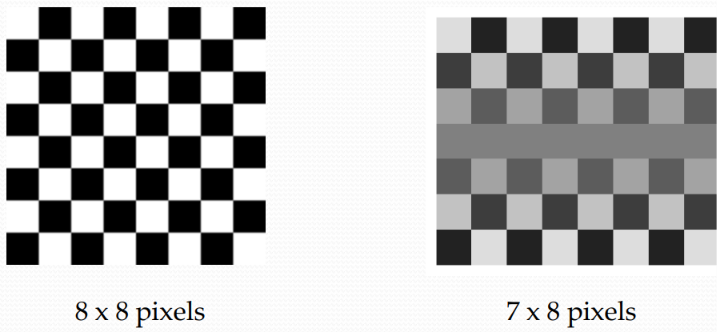
\includegraphics[width=0.6\textwidth]{figures/bicubic}
\end{figure}
\end{enumerate}